\documentclass[11pt]{article}
\usepackage[vietnamese]{babel}
\usepackage{sectsty}
\usepackage{graphicx}
\usepackage{setspace}
\usepackage{float} 

% Margins
\topmargin=-0.45in
\evensidemargin=0in
\oddsidemargin=0in
\textwidth=6.5in
\textheight=9.0in
\headsep=0.25in

\title{STROKE PREDICTION USING MACHINE LEARNING TECHNIQUES}
\author{Khổng Đức Quang - MSSV: 20225072}
\date{\today}

\begin{document}
	\maketitle
	
	\section{Tóm tắt}
	
	Đột quỵ là một tình trạng y tế khẩn cấp xảy ra khi dòng máu đến một phần não bị gián đoạn do xuất huyết hoặc tắc nghẽn bởi cục máu đông. Đây là nguyên nhân tử vong đứng thứ hai trên toàn cầu, với khoảng 5,5 triệu ca tử vong mỗi năm. Theo thống kê, mỗi năm có hơn 15 triệu người trên thế giới bị ảnh hưởng bởi đột quỵ, và trung bình cứ mỗi 4 phút lại có một trường hợp tử vong do tình trạng này.
	
	Phần lớn các trường hợp đột quỵ có liên quan chặt chẽ đến lối sống không lành mạnh, dẫn đến ước tính khoảng 80\% các trường hợp có thể được phòng ngừa. Do đó, việc xây dựng các mô hình dự đoán nguy cơ đột quỵ có ý nghĩa quan trọng trong việc ngăn chặn các tổn thương nghiêm trọng và giảm thiểu tỷ lệ tử vong liên quan. Công tác dự đoán không chỉ giúp cảnh báo sớm mà còn hỗ trợ trong việc đưa ra các biện pháp can thiệp kịp thời nhằm bảo vệ sức khỏe cộng đồng.
	
	\vspace{0.3cm}
	
	\section{Mục tiêu dự án}
	
	Mục tiêu của dự án này là dự đoán khả năng xảy ra đột quỵ não bằng cách ứng dụng các kỹ thuật học máy. Bằng cách phân tích dữ liệu y tế, em sẽ huấn luyện một số mô hình học máy nhằm nhận diện các mẫu và yếu tố rủi ro liên quan đến đột quỵ. Điều này sẽ hỗ trợ phát hiện sớm, cung cấp những thông tin quan trọng giúp đưa ra các biện pháp phòng ngừa và can thiệp kịp thời.
	\pagebreak
	
	\tableofcontents
	
	% Optional TOC
	% \tableofcontents
	% \pagebreak
	
	%--Paper--
	\pagebreak
	
	\listoffigures
	
	\pagebreak
	\section{Mô tả bộ dữ liệu}
	
	
	Bộ dữ liệu được em thu thập từ trang Web Kaggle để ước tính xem bệnh nhân có khả năng đột quỵ hay không. Đâu là bộ dữ liệu về thông tin của 5110 người bao gồm 11 thuộc tính và 1 cột stroke(output) là có khả năng đột quỵ hay không. (FEDESORIANO 2021). 
	
	Dưới đây là danh sách các thuộc tính:
	\begin{enumerate}
		\item Id (Interger Feature): Đây là dữ liệu kiểu số nhằm. Tuy nhiên thuộc tính này không làm ảnh hưởng tới Output nên em sẽ không phân tích thêm.
		\item Gender (Nominal Feature): Đây là thuộc tính kiểu chữ bao gồm các giá trị: Male, Female, Orther. Thuộc tính "Gender" (giới tính) có thể ảnh hưởng tới khả năng đột quỵ do sự khác biệt sinh học, nội tiết tố, và yếu tố hành vi giữa nam và nữ.
		\item Age (Interger Feature): Dữ liệu kiểu số. Thuộc này này là một yếu tố quan trọng ảnh hưởng đến khả năng đột quỵ.
		\item Hypertension (Integer Feature): Với hai giá trị khác nhau là: 0, 1.
		Đây là yếu tố nguy cơ lớn nhất đối với đột quỵ. Nó có ảnh hưởng sâu sắc đến khả năng đột quỵ.
		\item Heart Disease (Integer Feature): Với hai giá trị khác nhau là: 0, 1. Là một yếu tố có nguy cơ đáng kể gây đột quỵ. 
		\item Ever married (Boolean Feature): Với hai giá trị khác nhau là: True, False. Có thể liên quan đến nguy cơ đột quỵ qua các yếu tố gián tiếp, chẳng hạn như lối sống, sức khỏe tâm lý, và sự hỗ trợ xã hội.
		\item Work type (Nominal Feature): Có 5 loại giá trị khác nhau: Private, Self-employed, children, Govt-job, Never-worked. Và ảnh hưởng đáng kể đến nguy cơ đột quỵ thông qua các yếu tố như mức độ căng thẳng, hoạt động thể chất, và tiếp xúc với các yếu tố nguy cơ môi trường.
		\item Residence type (Nominal Feature): Có hai giá trị khác nhau là: Urban, Rural. Ảnh hưởng đến nguy cơ đột quỵ thông qua các yếu tố môi trường, điều kiện sống, và khả năng tiếp cận dịch vụ chăm sóc sức khỏe.
		\item Avg glucose level (Float Feature): Là một yếu tố quan trọng liên quan đến nguy cơ đột quỵ, đặc biệt thông qua mối liên hệ với bệnh tiểu đường và rối loạn chuyển hóa. Mức đường huyết bất thường, cả cao lẫn thấp, đều có thể làm tăng nguy cơ đột quỵ.
		\item BMI (Float Feature): Là một chỉ số quan trọng để đánh giá mức độ béo phì hoặc thừa cân của một người, và nó có mối liên hệ mạnh mẽ với nguy cơ đột quỵ.
		\item Smoking status(Nominal Feature): Với 4 giá trị khác nhau: Never smoked, Unknown, formerly smoked, smokes. Là một yếu tố nguy cơ quan trọng đối với nhiều bệnh lý, bao gồm đột quỵ. Hút thuốc lá ảnh hưởng đến sức khỏe của tim và mạch máu, gây ra những tác động tiêu cực trực tiếp làm tăng nguy cơ đột quỵ. 
	\end{enumerate}
	
	\pagebreak
	
	\section{Xử lý dữ liệu}
	
	Trong quá trình tiền xử lý số liệu, em nhận thấy có các vấn đề sau cần xử lý:
	\begin{enumerate}
		\item Đầu tiên em \textbf{loại bỏ đi cột ID} do cột này không ảnh hưởng tới khả năng đột quỵ.
		\item
		\textbf{Xử lý các giá trị NULL}
		\begin{figure}[H]
			\centering
			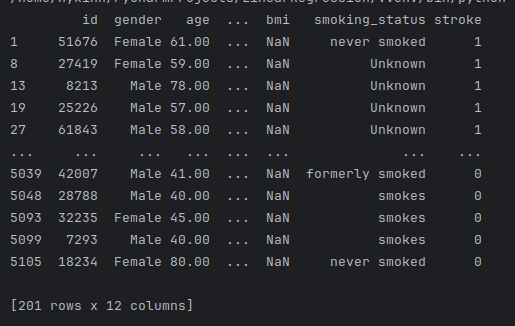
\includegraphics[width=0.7\linewidth]{nullCheck}
			\caption{Kiểm tra giá trị NULL}
			\label{fig:nullcheck}
		\end{figure}
		Sau khi kiểm tra em nhận thấy cột thuộc tính "bmi" có 201 giá trị NULL. Để xử lý vấn đề này có ba phương pháp phổ biến: Xóa các dòng chứa giá trị NULL, Điền giá trị trung bình hoặc trung vị, Điền giá trị dựa trên mô hình (Model-based Impution).
		Sau khi tìm hiểu ưu và nhược điểm của từng phương pháp em quyểt định lựa chọn cách điền giá trị trung bình là lựa chọn vừa đơn giản vừa hiệu quả, giúp giữ được lại toàn bộ dữ liệu mà không làm giảm kích thước bộ dữ liệu.
		\item Bước tiếp theo là \textbf{chuyển đổi dữ liệu kiểu Categorical thành dữ liệu kiểu Numerical}. Phương pháp Hash e Encoding và One-hot Encoding được sử dụng để thực hiện các bước chuyển đổi này.
		\item \textbf{Phân chia dữ liệu}: Em chia bộ dữ liệu thành hai tập là: tập huấn luyện(80\%), tập kiểm tra(20\%) bằng cách sử dụng hàm train\_test\_split được cung cấp trong thư viện scikit-learn
		\item \textbf{Feature scaling (chuẩn hóa đặc trưng)} là bước cuối cùng
		%--/Paper--
	\end{enumerate}
	\pagebreak
	
	\section{Phân tích dữ liệu}
	
	\begin{figure}[H]
		\centering
		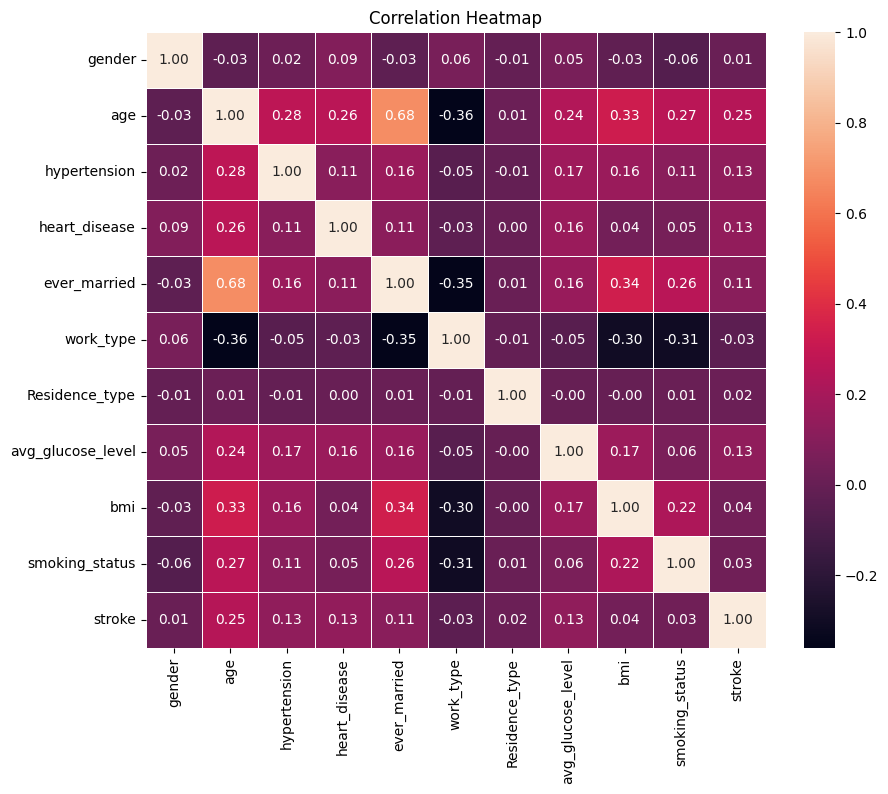
\includegraphics[width=0.7\linewidth]{correlationHeatmap}
		\caption{Correlation Heatmap}
		\label{fig:correlationheatmap}
	\end{figure}
	Nhận xét:
	
	
	\begin{flushleft}
		- Một số tương quan dương mạnh:
		
		+) Age và evernhất\_married (0.68) có tương quan dương mạnh nhất
		
		+) Age cho thấy mối tương quan tích cực vừa phải với BMI (0.33), Hypertension (0.28) và smoking\_status (0.27)
		\vspace{0.2cm}
		
		- Một số tương quan yếu đáng chú ý:
		
		+) Work\_type có một số tương quan yếu với: age (-0.36), ever\_married (-0.35), bmi (-0.30), smoking\_status (-0.31)
		\vspace{0.2cm}
		
		- Tương quan đột quỵ:
		
		+) Stroke có tương quan yếu hoặc trung bình yếu với hầu hết các thuộc tính trong bảng.
		
		+) Age có tương quan cao nhất nhưng vẫn là tương quan yếu với Stroke (0.25), tương tự là heart\_disease và hypertension, cả hai đều là 0.13
		\vspace{0.2cm}
		
		- Hầu hết các tương quan đều là yếu và rất yếu, gần giá trị 0
		\vspace{0.2cm}
		
		\textbf{Tóm lại}, age là yếu tố có ảnh hưởng lớn nhất đến khả năng đột quỵ.
	\end{flushleft}
	
	\begin{figure}[H]
		\centering
		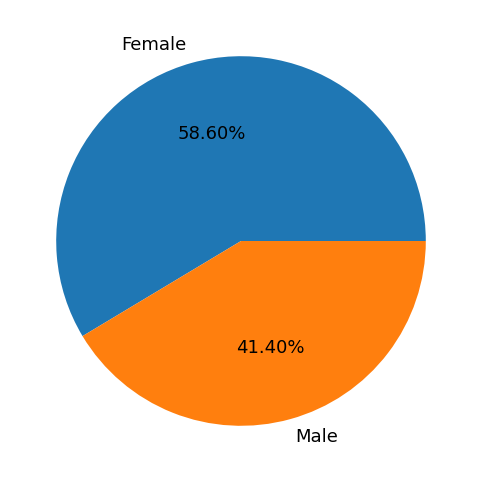
\includegraphics[width=0.5\linewidth]{genderPie}
		\caption{Biểu đồ gender}
		\label{fig:genderpie}
	\end{figure}
	
	\begin{figure}[H]
		\centering
		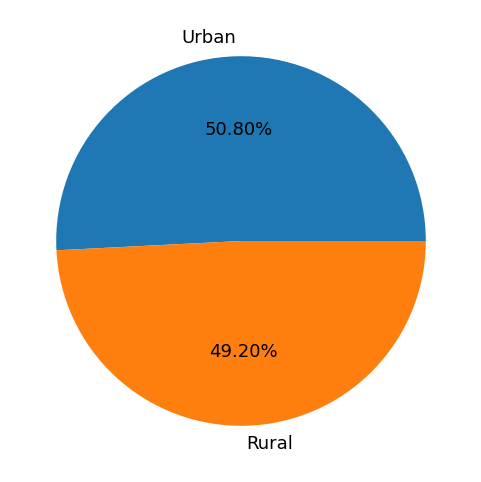
\includegraphics[width=0.5\linewidth]{residencePie}
		\caption{Biểu đồ residencetype\_type}
		\label{fig:residencepie}
	\end{figure}
	
	\begin{figure}[H]
		\centering
		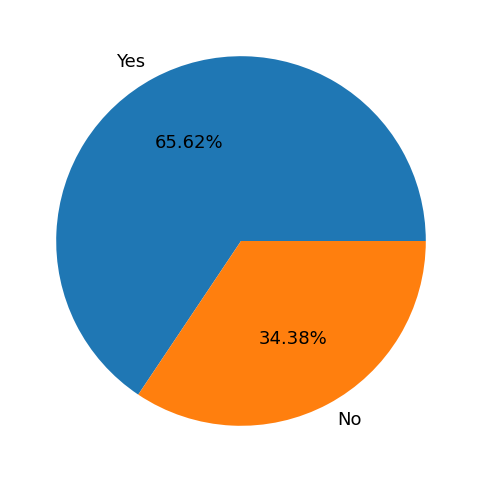
\includegraphics[width=0.5\linewidth]{marriedPie}
		\caption{Biểu đồ ever\_married}
		\label{fig:marriedpie}
	\end{figure}
	
	\begin{figure}[H]
		\centering
		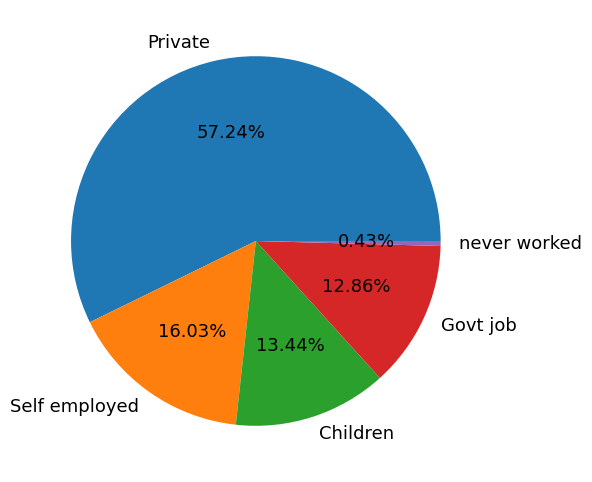
\includegraphics[width=0.5\linewidth]{workedPie}
		\caption{Biểu đồ work\_type}
		\label{fig:workedpie}
	\end{figure}
	
	\begin{figure}[H]
		\centering
		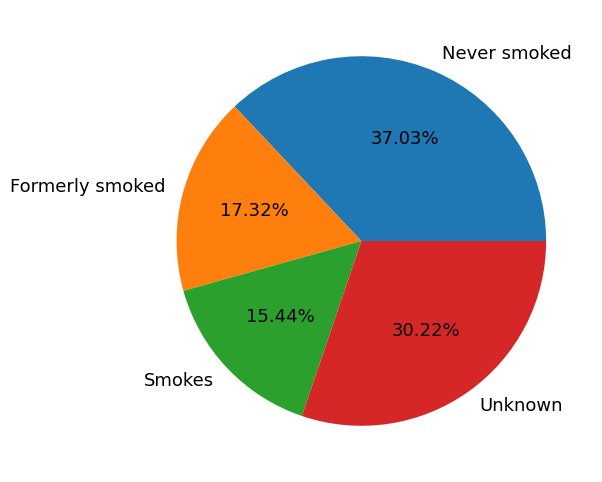
\includegraphics[width=0.5\linewidth]{smokingPie}
		\caption{Biểu đồ smoking\_status}
		\label{fig:smokingpie}
	\end{figure}
	
	\begin{figure}[H]
		\centering
		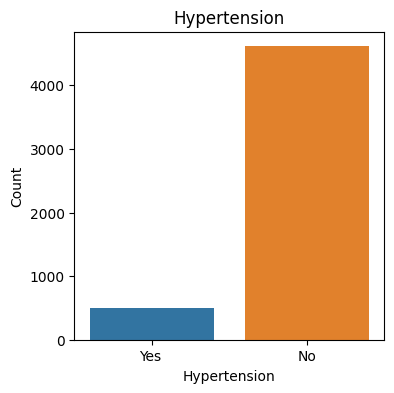
\includegraphics[width=0.5\linewidth]{hypertensionChart}
		\caption{Biểu đồ hypertension}
		\label{fig:hypertensionchart}
	\end{figure}
	
	\begin{figure}[H]
		\centering
		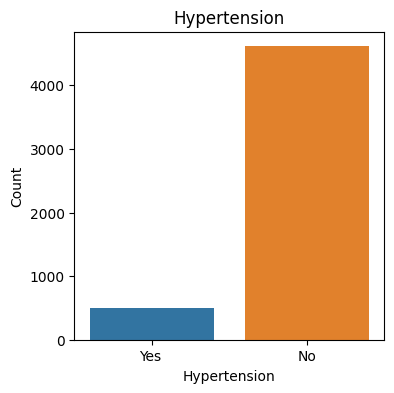
\includegraphics[width=0.5\linewidth]{hypertensionChart}
		\caption{Biểu đồ heart\_disease}
		\label{fig:hypertensionchart}
	\end{figure}
	
	\begin{figure}[H]
		\centering
		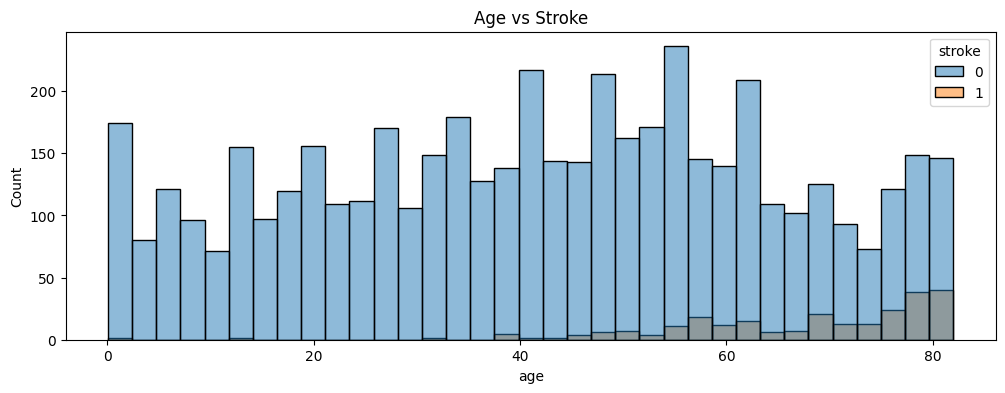
\includegraphics[width=1.0\linewidth]{ageAndStroke}
		\caption{Biểu đồstroke liên hệ age và stroke}
		\label{fig:ageandstroke}
	\end{figure}
	
	\textbf{Age và Stroke}:
	\begin{enumerate}
		\item Các trường hợp đột quỵ tăng dần sau 40 tuổi.
		\item Tỷ lệ đột quỵ cao nhất nằm trong độ tuổi từ 60-80 tuổi.
		\item Có rất ít trường hợp đột quỵ dưới 40 tuổi.
		\item Phân bố cho thấy tuổi tác là yếu tố có ảnh hưởng đáng kể đối với đột quỵ.
	\end{enumerate}
	
	
	\begin{figure}[H]
		\centering
		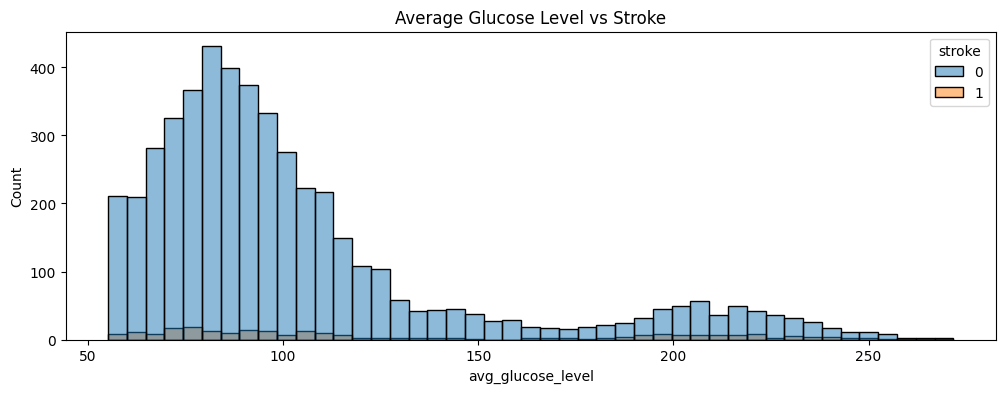
\includegraphics[width=1.0\linewidth]{glucoseAndStroke}
		\caption{Biểu đồ liên hệ average\_glucose\_level}
		\label{fig:glucoseandstroke}
	\end{figure}
	
	\textbf{Average\_glucose\_level và Stroke}S:
	\begin{enumerate}
		\item Các trường hợp đột quỵ có xu hướng xuất hiện nhiều hơn ở các mức đường huyết trung bình cao hơn, đặc biệt từ 120 mg/dL trở lên.
		\item Trong phạm vi đường huyết từ 180 mg/dL đến 250 mg/dL, tỷ lệ người bị đột quỵ tăng lên đáng kể, dù số lượng tổng thể thấp hơn.
		\item Ở mức đường huyết dưới 100 mg/dL, tỷ lệ đột quỵ thấp hơn rõ rệt.
	\end{enumerate}
	
	
	\begin{figure}[H]
		\centering
		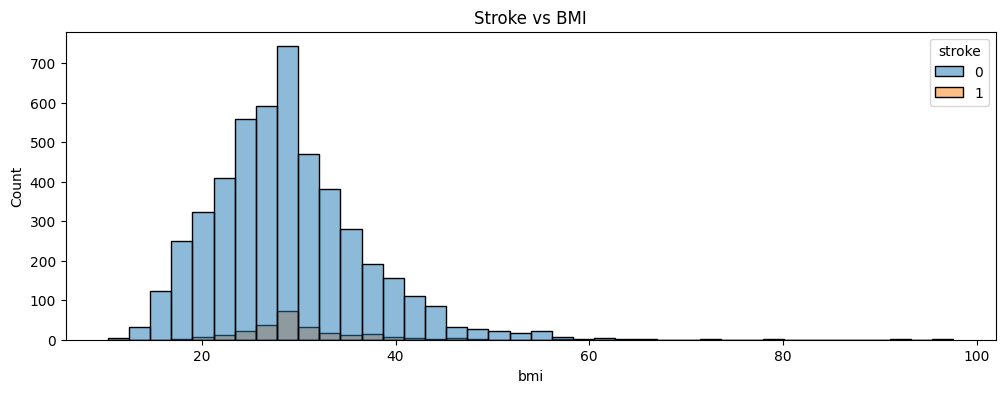
\includegraphics[width=1.0\linewidth]{bmiAndStroke}
		\caption{Biểu đồ liên hệ bmi và stroke}
		\label{fig:bmiandstroke}
	\end{figure}
	
	
	\textbf{BMI và Stroke}:
	\begin{enumerate}
		\item Phần lớn mọi người có chỉ số BMI từ 20-40.
		\item Phân bố đỉnh nằm trong khoảng 25-35.
		\item Các trường hợp đột quỵ (màu xám) xuất hiện thường xuyên hơn ở nhóm thừa cân và béo phì (BMI > 25).
		\item Dữ liệu cho thấy tình trạng thừa cân hoặc béo phì có thể làm tăng nguy cơ đột quỵ, mặc dù mối quan hệ này có vẻ ít nghiêm trọng hơn so với tuổi tác hoặc lượng đường trong máu.
	\end{enumerate}
	
	\section{Xem xét sự mất cân bằng dữ liệu}
	
	\begin{figure}[H]
		\centering
		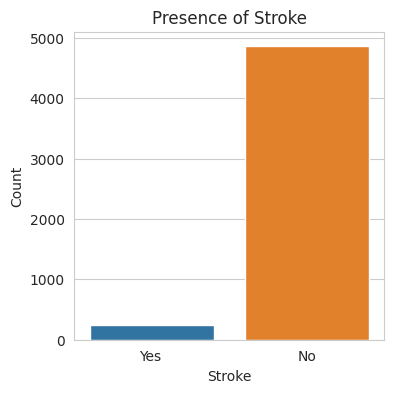
\includegraphics[width=0.5\linewidth]{dataBalanceCompare}
		\caption{Biểu đồ so sánh số lượng người đột quỵ và không đột quỵ}
		\label{fig:databalancecompare}
	\end{figure}
	
	\begin{figure}[H]
		\centering
		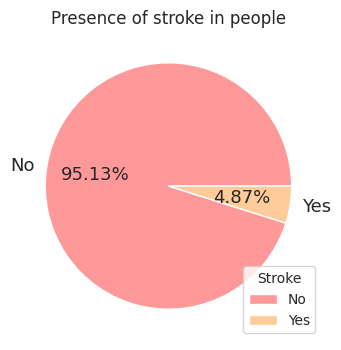
\includegraphics[width=0.5\linewidth]{compareBalancePie}
		\caption{Phân bố tỷ lệ người có và không đột quỵ}
		\label{fig:comparebalancepie}
	\end{figure}
	
	\textbf{Nhận xét}:
	\begin{enumerate}
		\item Mất cân bằng dữ liệu nghiêm trọng. Tỷ lệ người không bị đột quỵ (No) chiếm 95.13\% tổng số dữ liệu. Trong khi đó, tỷ lệ người bị đột quỵ (Yes) chỉ chiếm 4.87\%. Điều này cho thấy dữ liệu mất cân bằng nghiêm trọng giữa hai nhóm.
		\item Việc mất cân bằng dữ liệu này có thể dẫn đến việc mô hình học máy thiên vị, tập trung vào việc dự đoán chính xác lớp chiếm đa số (No) mà bỏ qua lớp thiểu số (Yes). \textbf{Từ đó dẫn đến kết quả} mô hình có thể đạt độ chính xác cao nhưng không phát hiện chính xác các trường hợp bị đột quỵ, làm tăng tỷ lệ False Negative (bỏ sót những người thực sự bị đột quỵ).
	\end{enumerate}
	
	\textbf{Giải pháp}:
	\begin{flushleft}
		Đề giải quyết vấn đề trên cũng như cải thiện khả năng dự đoán của mô hình, em sẽ áp dụng kỹ thuật xử lý dữ liệu mất cân bằng đó là Oversampling: Tăng số lượng mẫu cho lớp thiểu số bằng cách sử dụng SMOTE.
		
		\begin{figure}[H]
			\centering
			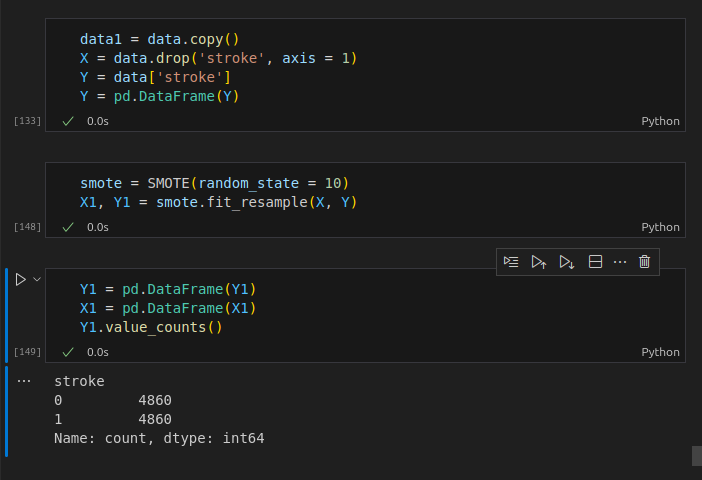
\includegraphics[width=0.7\linewidth]{solBalanceData}
			\caption{Xử lý dữ liệu mất cân bằng}
			\label{fig:solbalancedata}
		\end{figure}
		
		Sau khi sử dụng kỹ thuật SMOTE để xử lý sự mất cân bằng của dữ liệu thì số trường hợp đột quỵ và không đột quỵ đã bằng nhau như kết quả trên hình.
	\end{flushleft}
	
	%\section{Huấn luyện mô hình}
	
	%\subsection{LogisticRegression}
	
	
\end{document}